\documentclass[11pt,oneside]{article}
\usepackage{graphicx}
\begin{document}

\title{CS4310 - Design \& Analysis of Algorithms\\Assignment 1}
\author{Alex Dekau}
\date{September 9\textsuperscript{th}, 2016}
\maketitle
\tableofcontents

\section{Introduction}
I'm Alex Dekau and I'm an undergraduate student in the Computer Science program here at Western. I am currently a junior and enjoy watching sports, mainly baseball and soccer. I also enjoy playing video games in my free time. I currently work over at the University Computing Center as a student employee.

\subsection{What I Hope to Gain From This Class}
I hope to learn how to analyze my own code and make sure that it runs as efficiently as possible without having to rely on the compiler optimizing my code. I believe that it is a useful function of a compiler, but relying on it too heavily leads to lazy coding and less maintainable code in the future. I have not decided yet if I want to pursue a graduate degree. I'm not sure how useful it would be for what I want to be as a programmer. I'm not sure what the ``research" part of programming implies.

\subsection{Future Goals}
I would like to apply what I learn to my future work and open source projects. I've always used open source software since in my opinion it leads to better software through community collaboration, and would like to eventually be a contributor to a few projects to return the favor. I would like to be the best programmer that I can be so I can help other people out with programming in places such as Stack Overflow. For my plans on where I'd like to work, I'd say I would like to get a job programming here at Western since so many people have told me that it's a great place to work for. 


\section{Picture}
\begin{center}
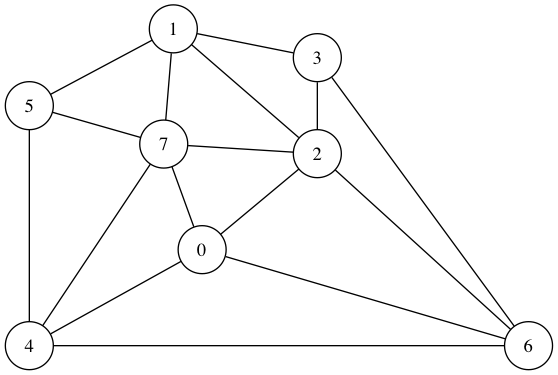
\includegraphics[scale=0.75]{graph.png}
\end{center}


\end{document}